\chapter{Processing the Captured Data}
This chapter is dedicated to the complex process of extracting critical data from the video files. The following digram shows the process of converting a data heavy video file to a more lightweight .csv (Comma Separated Values) file.

\section{Processing the IMU Data}

\subsection{Capture IMU Data}
To use the smartphone as an IMU a free application "AndroSensor" \cite{androsensor} was installed. This application could log parameter from all the  sensor s and could be configured in various ways

\begin{figure}[!ht] 
\captionsetup{width=\linewidth, font=small}  
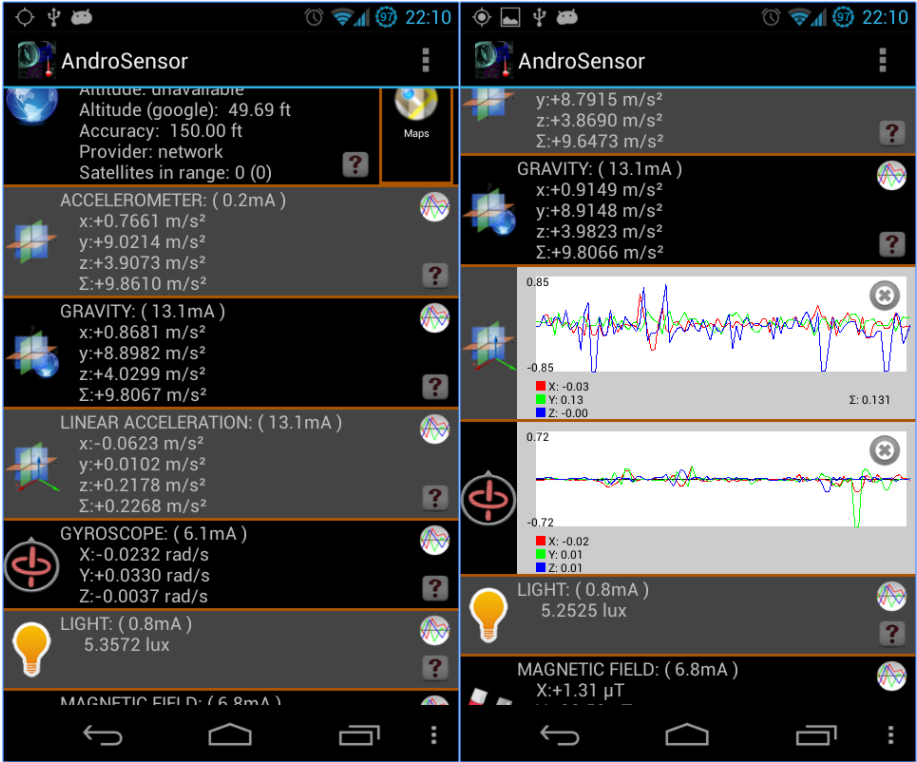
\includegraphics[width=\linewidth]{figures/as.png}
\caption{Androsensor Screenshots from \cite{androsensor}}
\label{fig:as}
\end{figure}


The IMU data logged by the smartphone was saved as a .CSV file with the first row containing the headings of various variables. These headings were

\begin{table}
\centering
\caption{My caption}
\label{my-label}
\begin{tabular}{ll}
Heading               & Fields  \\
ACCELEROMETER       & X,Y,Z  \\
GRAVITY              & X,Y,Z \\
LINEAR ACCELERATION  & X,Y,Z\\
GYROSCOPE            & X,Y,Z \\
MAGNETIC FIELD       &  X,Y,Z\\
ORIENTATION          &  X,Y,Z\\
ATMOSPHERIC PRESSURE  &  \\
LOCATION Latitude     &  \\
LOCATION Longitude    &  \\
LOCATION Speed        &  \\
LOCATION ORIENTATION  & 
\end{tabular}
\end{table}

All these variables have been recorded with respect the smartphone frame of reference as shown below
\begin{figure}[!ht] 
\captionsetup{width=\linewidth, font=small}  
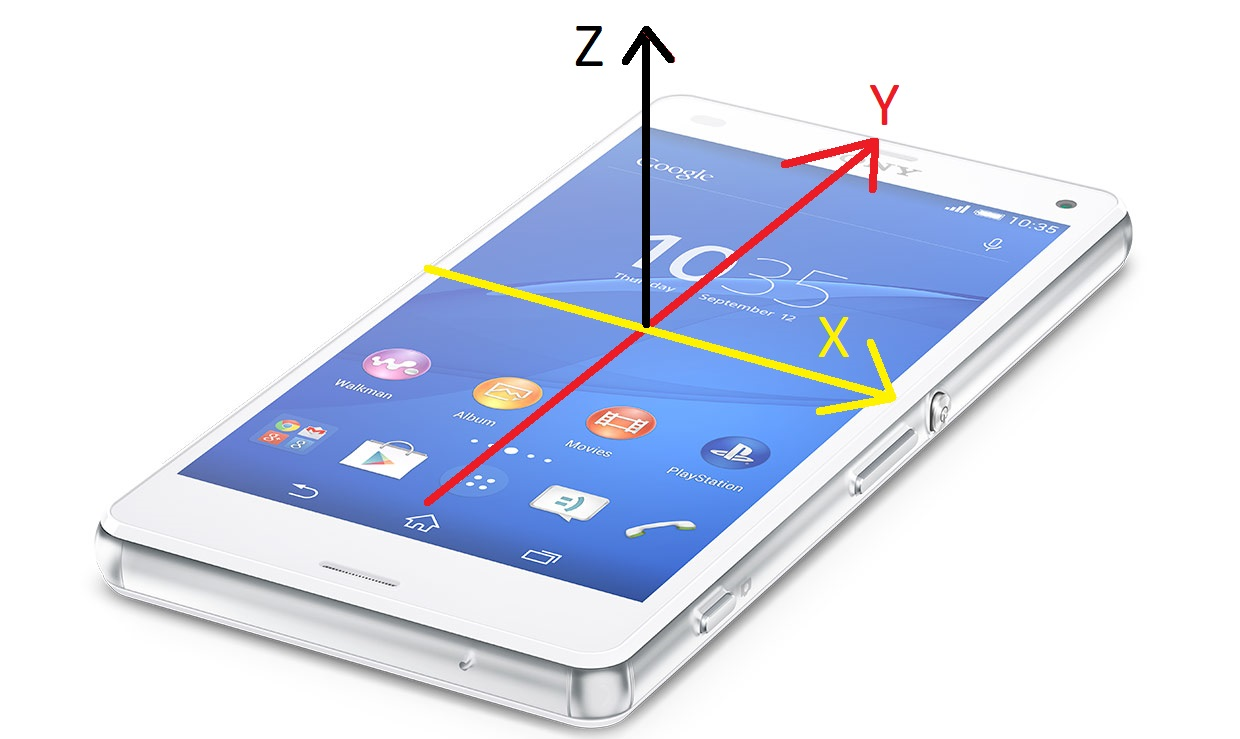
\includegraphics[width=\linewidth]{figures/phone.jpg}
\caption{Figure demonstrating the frame of reference of the smartphone}
\label{fig:phone}
\end{figure}










\section{Processing the Video Data}
The following flowcharts depicts the procedural processing of video data.
\begin{figure}[!ht]
  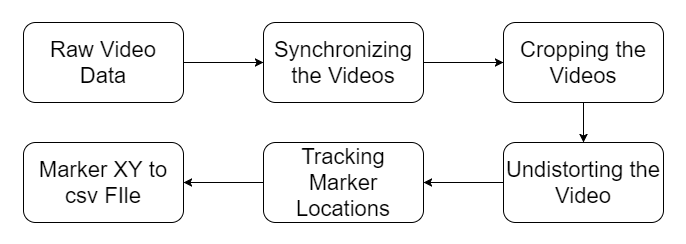
\includegraphics[width=\linewidth]{figures/videoProcess.png}
  \caption{Diagram showing the progression and dependence of the major stages of video processing in the project}
  \label{fig:videoProcess}
\end{figure}

\subsection{Obtaining Video Data}
Using the chest mounted cameras detailed in the previous chapter we can generate raw video data. The GPHS cameras can be configured to record at different frame rates and resolutions as discussed in the previous chapter. The video files where stored in an .MP4 format. This meant that during recording the video was compressed and the 


\subsection{Synchronizing Video Sources}
I typical problem faced when working with different sources of data is that of synchronization. Since this project used 4 different cameras, synchronizing the video sources are critical to generate accurate stereo vision data.

The problem of synchronization was overcome by using a audio cue to align the video data post capturing. With all systems recording, a simple hand clap can serve as a spiking audio input easily identified in the audio track of the video streams. The frame associated with this audio spike can be identified using SVP (Sony Vegas Pro) video editing software as shown in the figure below. 

\begin{figure}[!ht]
\centering
  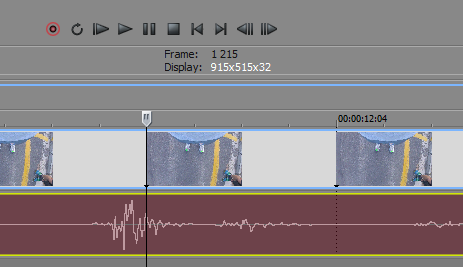
\includegraphics[width=0.5\linewidth]{figures/svpframe.png}
  \caption{Figure showing the user interface of SVP video editing software}
  \label{fig:svpframe}
\end{figure}

The red track in the above figure shows the recorded audio stream while the corresponding frames are displayed in the blue track above that. The cursor is aligned with the audio spike caused by the clap with the corresponding frame number displayed below the playback controls.

This method was repeated for every video stream such that a common starting point was generated. 

\subsection{Cutting Critical Video Data}

With the video data synchronized the next step was to generate a subset of video demonstrating a transient period and steady state period of running. From accelerometer readings we can easily determine the gait cycle period of our subject; that is the amount of time take between the same foot impacting the ground. These impacts are visible as spikes as seen in the accelerometer data.  

\subsection{Undistorting the Video Data}
To generate accurate distances using stereo vision the video frames need to be undistorted.

Distortion of the frames is a result of the 

\cite{Hartley2004} 

\subsection{Tracking and Exporting Marker Positions in the Frame}

using work from \cite{hedrick2008software}












